\chapter{Implementation}\label{sec:implementation}


This section describes the reference implementation for the conceptual framework in Chapter \ref{cha:concept}.
First, the general architecture is explained.
Various components and interaction techniques of the geographical visualization are detailed.
The integration of the geographical visualization in the existing \visan{} is shown.
The connection of the conceptual framework and the implemented framework is examined.

\section{Architecture}

% \begin{figure}[h!]
%   \centering
%   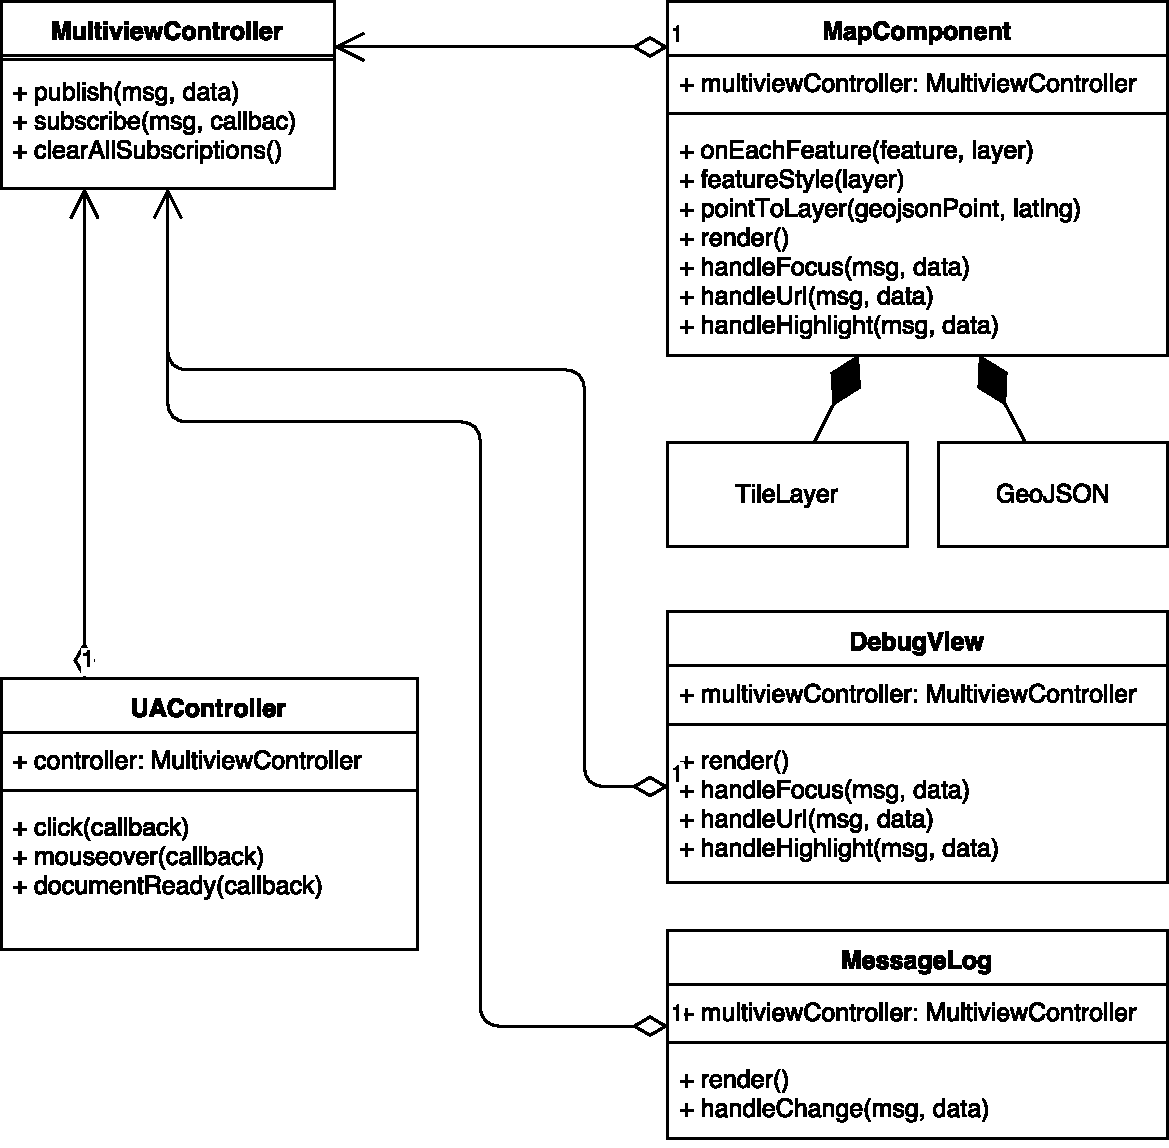
\includegraphics[width=\textwidth]{figures/implementation/thesis-class-diagram.pdf}
%   \caption{%
%     Class diagram of the most important components and their relations
%   }\label{fig:implementation:class-diagram}
% \end{figure}

\begin{figure}[h!]
  \centering
  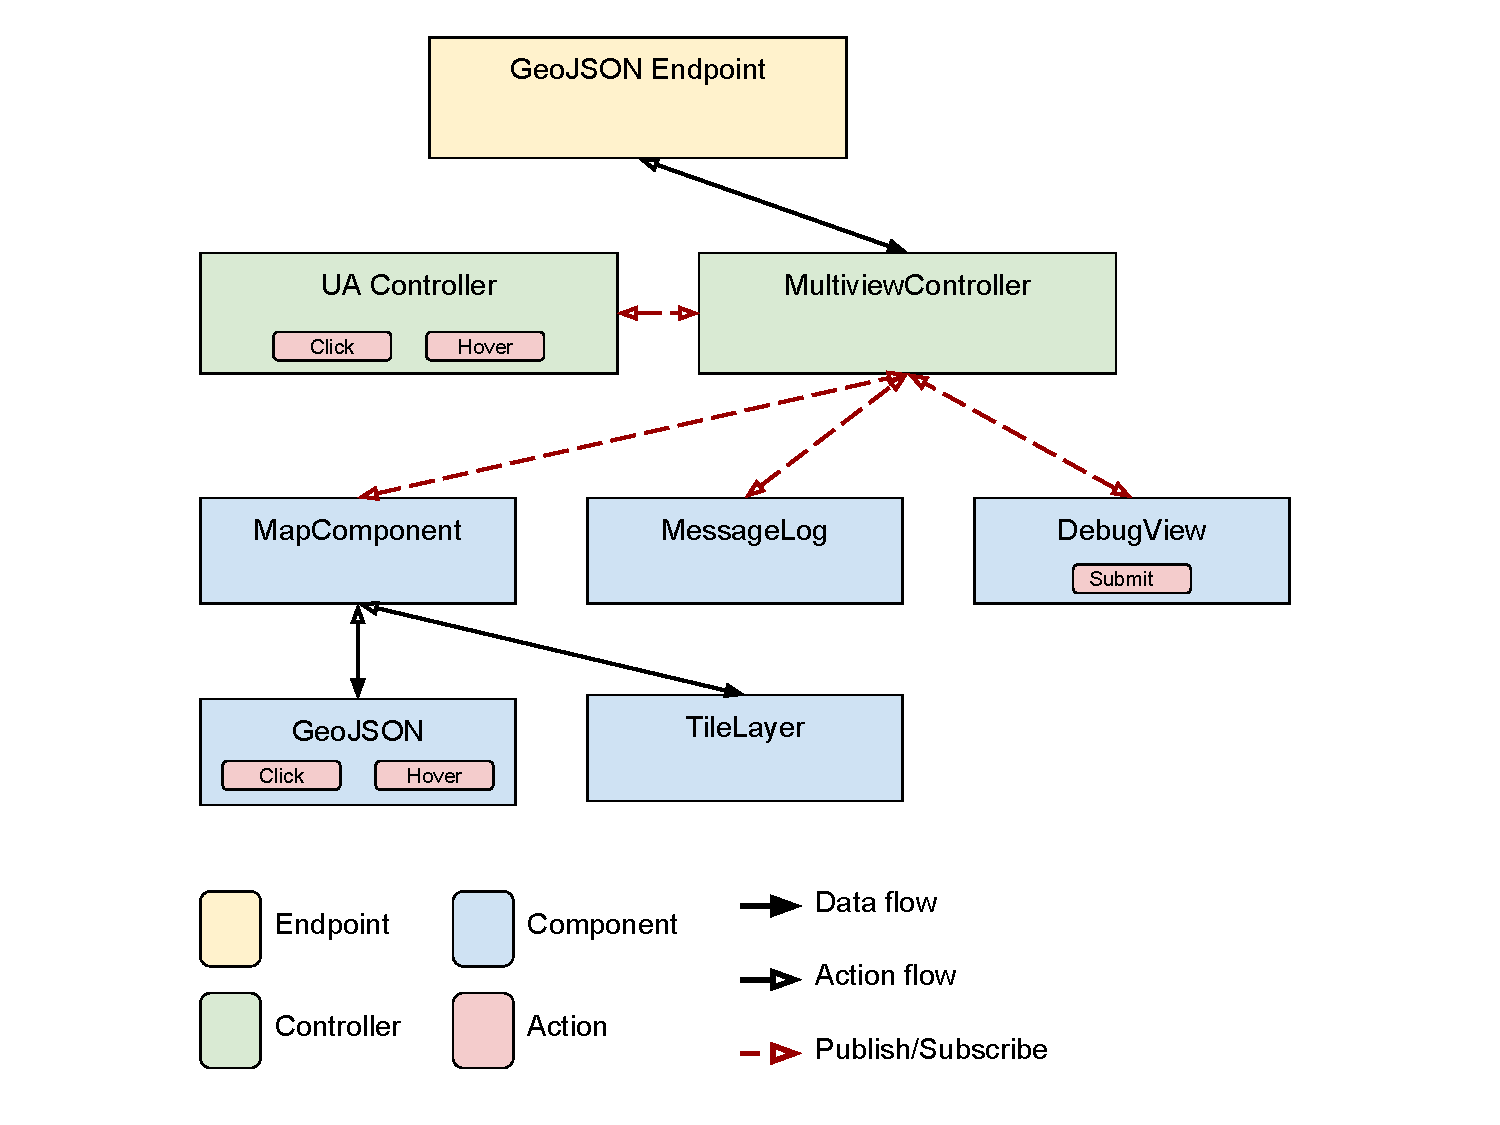
\includegraphics[width=\textwidth]{figures/implementation/thesis-architecture.pdf}
  \caption{%
    Architecture of the reference implementation.
  }\label{fig:implementation:architecture}
\end{figure}

The reference implementation of the conceptual framework is written in \attr{TypeScript} and uses \attr{PubSubJS} for communication.
The visualizations are implemented with \attr{React} and the geographical visualization uses \attr{Leaflet} under the hood.
Geometry data is exchanged with \attr{GeoJSON} as data format.

The general architecture of the reference implementation is shown in Figure~\ref{fig:implementation:architecture}.
Within the existing \visan{} the \attr{UAController} controls the rendering of the \tmap{}.
The rendering of the geographical visualization is controlled by the \attr{MapComponent}.
Additionally, there are two other views, \attr{DebugView} and \attr{MessageLog}.
These views record interactions at runtime and can trigger and simulate an interaction.

Every view has a reference to \attr{MultiviewController} in order to subscribe to interactions.
The \attr{MultiviewController} itself does not have a visual representation.

The classes \attr{MapComponent}, \attr{DebugView} and \attr{MessageLog} are implemented with React and have a \attr{render} method.
This way, these class can be initialized and rendered anywhere in the DOM tree.
They are dependency free, except of the reference to a \attr{MultiviewController}, which makes those classes easy to test.

The views that are implemented with React automatically re-render if their internal state changes.
Event handlers just have to publish an interaction, if the view is subscribed to the same interaction, it will automatically re-render.

\section{Software patterns}\label{sec:implementation:patterns}
Figure~\ref{fig:implementation:sequence-diagram} shows how \cmvs{} can be automatically updated even if the environment lacks a native update-mechanism.

\begin{figure}[h!]
  \centering
  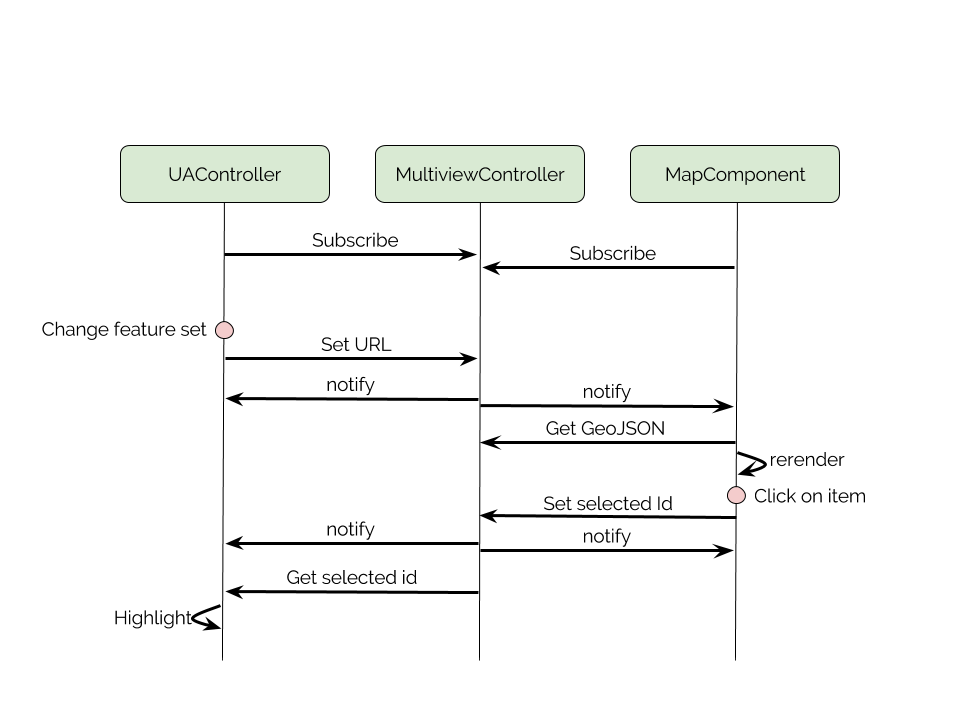
\includegraphics[width=\textwidth]{images/sequence-diagram.png}
  \caption{%
    The sequence diagram shows the notification of different components.
  The user first chooses a feature set and hovers over a polygon in the geographical map.
  }\label{fig:implementation:sequence-diagram}
\end{figure}


\textbf{The Observer pattern} allows multiple \emph{observers} to react to changes of an observed state.
In our case, the observed state is the \attr{MultiviewController}.
Any change to the \attr{MultiviewController} will subsequently be broadcasted to all connected views.


\textbf{Publisher subscriber}
In our particular case we apply a special form of the observer pattern, the so called ``Publish-subscribe'' pattern\cite{Eugster2003}.
Publish-subsribe is a messaging pattern which is widely used in message queues.
In this scenario, senders of messages simply categorize their messages which will be consumed by subscribers of the category.
The scenario has very low coupling, publishers do not even need to know the existence of subscribers.

\textbf{Component pattern}
State-of-the-art javascript component frameworks like ReactJS and EmberJS follow the component pattern for the architecture of a single page web application.
The component pattern imposes a hierarchical structure on a website.
Each component is responsible for a task and may contain other components.
The components are joined at the root node of the page.

This pattern is very applicable to \cmvs{}.
The different views of \cmvs{} share state, i.e.\ the feature, that is currently highlighted or the applied filter on the data.
So the views are components and their closest common ancestor is the \cmv{} itself, controlling state and passing user interaction down to it's children.

\begin{figure}[h!]
  \centering
  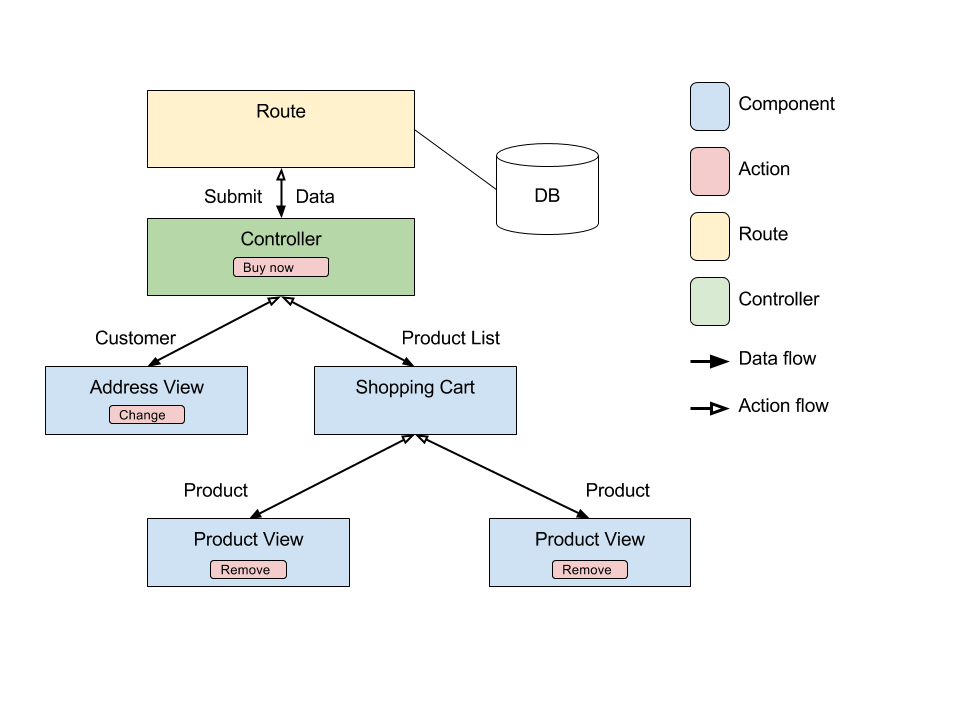
\includegraphics[width=\textwidth]{images/data-down-actions-up.png}
  \caption{%
    Implementation of the component pattern in EmberJS\@.
    The example shows a page of a webshop.
    The customer is about to order the items in the shopping cart.
  }\label{fig:implementation:data-down-actions-up}
\end{figure}

\textbf{Actions up --- Data down}

Version 2.0 of Ember introduced a common phrase how to use this pattern effectively: ``Data down, actions up''\cite{Emberigniter2017}
In the domain of \cmvs{} actions would mean user interactions, e.g.\ a click on a feature.
The action will notify the controlling \cmv{} component.
Actions may change data, and the changes will be passed to to all dependen views.
These views are then rerendered.

Examples for the kind of data that might trigger a rerendering of a view:
\begin{itemize}
  \item
    The selected feature or a list of selected features
  \item
    A list of thresholds for certain features as a filter
\end{itemize}


\section{Geographical visualization with React and Leaflet}

The geographical visualization is implemented as a \attr{Map} component of the React Leaflet library.
Listing \ref{lst:implementation:render} shows the \attr{render} method of the component.

\lstinputlisting[
  language=JavaScript,
  label={lst:implementation:render},
  caption={\attr{render} method of the Map component of the geographical visualization}
]{listings/implementation/render.tsx}

The \attr{render} method is the only required method of a React component.
It will be invoked on the initial rendering of the component of the \attr{DOM} and on every update of the component's properties.
React's templating language ``\attr{JSX}'' allows to nest other child components in to the React parent component.
In this case the \attr{Map} component includes a \attr{TileLayer} \attr{GeoJSON} component from the \attr{react-leaflet} library.
This library conveniently provides ``React components for Leaflet maps.''~\cite{ReactLeaflet2017}.

\subsection{GeoJSON component}

The \attr{GeoJSON} component is provided by the \attr{Map} component with a couple of properties:
It gets a
\begin{enumerate*}[label=(\arabic*)]
  \item
    geojsonURL as well as a
  \item
    geojson as data attribute. Furthermore a couple of callbacks is passed into the child component, including
  \item
    featureStyle,
  \item
    pointToLayer and
  \item
    onEachFeature.
\end{enumerate*}

This way, the parent \attr{Map} component controls the data flow and without a \attr{geojson} object, no polygons are placed on the map.
A changed \attr{geojsonURL} will always update the child component as it is used a \attr{key} on the \attr{GeoJSON} component.
The callbacks passed into the \attr{GeoJSON} component control the visual representation of each polygon and they add event handlers for a mouse click or a mouse move on each polygon.
Listing \ref{lst:implementation:onEachFeature} shows the event handlers added to the map.

\lstinputlisting[
  language=JavaScript,
  label={lst:implementation:onEachFeature},
  caption={\attr{onEachFeature} callback, adding handlers for mouse events}
]{listings/implementation/onEachFeature.tsx}

First we cache all layers in the internal state of the \attr{Map} component.
On each \attr{mouseover} event, the \attr{id} of the feature is published as \attr{mcv.select.highlight} interaction.
A \attr{click} event is distinguised if the control key is pressed or not.
In the latter case, the id of the feature is either added or removed from the list of focused ids and then the list of focused ids is published as \attr{mcv.select.focus} interaction.

\lstinputlisting[
  language=JavaScript,
  label={lst:implementation:featureStyle},
  caption={\attr{featureStyle} callback, configuring the visual appearance depending on the currently highlighted or focused feature ids}
]{listings/implementation/featureStyle.tsx}

The \attr{featureStyle} in Listing \ref{lst:implementation:featureStyle} method is very straightforward.
If the feature is currently focused, the \attr{fillColor} of the polygon is red, otherwise blue.
Likewise, if the feature is currently highlighted, the polygon has a white, solid stroke.

\lstinputlisting[
  language=JavaScript,
  label={lst:implementation:pointToLayer},
  caption={\attr{pointToLayer} callback, if a feature of \attr{GeoJSON} has a point geometry, it will be shown as a circle}
]{listings/implementation/pointToLayer.tsx}

Finally, we configure how to display point geometries in callback \attr{poinToLayer}.
Since normal markers do not have a configurable color and style, we instruct the \attr{GeoJSON} component to render a \attr{CircleMarker} for each point geometry instead.
This way, the same options of \attr{featureStyle} can be applied to both point and area geometries.

\section{MultiviewController}

The \attr{MultiviewController} is a simple wrapper around the library \attr{PubSubJS} and works as a broker for interactions across \cmvs{}.


As the central part of the software, the \attr{MultiviewController} is also used for certain performance optimiziations.
These optimizations affect how often the geometries are reloaded, i.e.\ it reduces the number of requests to the \attr{GeoJSON} endpoint.


\lstinputlisting[
  language=JavaScript,
  label={lst:implementation:multiviewController},
  caption={The \attr{multiviewController} avoids unnecessary requests to reload geometries}
]{listings/implementation/multiviewController.tsx}

As shown in Listing~{list:implementation:multiviewController}, the geometries depend on a change of the \attr{url} of the geometries.
A change of the \attr{url} will automatically trigger an interaction of type \attr{reconfigure} to reload geometries.

An example of these geometries can be seen in listing~\ref{lst:geojson:example}.
For convenience, the file includes the aggregated data in the \attr{properties} of each feature.
In this case the colors the shapes of the \tmap{} are based on the value of \attr{user_count_normalized}.
Each feature comes with a unique \attr{id} which is published when a user interacts with the feature.

\lstinputlisting[
  language=JavaScript,
  label={lst:geojson:example},
  caption={A truncated example of a user distribution across German federal states}
]{listings/example.geojson}

We can use this data as input for our common \visan{}, e.g.\ figure~\ref{fig:implementation:user_distribution} shows the user distribution of \rufu{}.

\begin{figure}[h!]
  \centering
  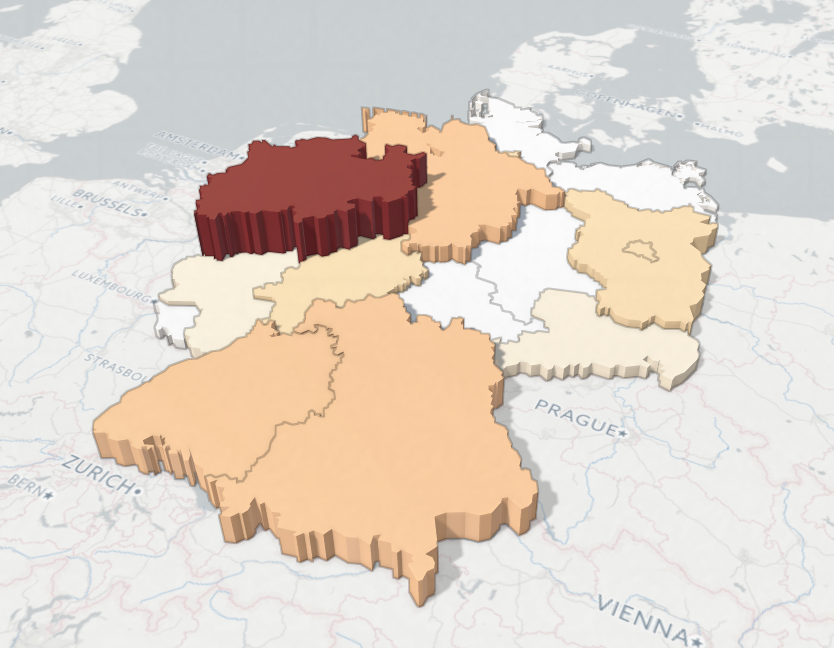
\includegraphics[width=\textwidth]{images/ua_example.png}
  \caption{%
    User distribution of \rufu{} across German federal states
  }\label{fig:implementation:user_distribution}
\end{figure}




\section{Implemented interactions}

In the course of this thesis we want to implement the following interactions:
\begin{itemize}
  \item
    \emph{Select}: The user clicks on a building or region in a geographical map and all affected properties in the \tmap{} will be highlighted.
  \item
    \emph{Explore}: The user clicks on a block in the \tmap{} and the viewpoint in the geographical map will be centered on relevant area.
  \item
    \emph{Reconfigure}: The user selects a different feature set and the changes are reflected in both the geographical map (e.g. point instead of polygon geometries) and in the \tmap{}.
  \item
    \emph{Filter}: The user double-clicks on a region in a geographical map and the \tmap{} will be based on data of only that region.
\end{itemize}
